%%%%%%%%%%%%%%%%%%%% author.tex %%%%%%%%%%%%%%%%%%%%%%%%%%%%%%%%%%%
%
% sample root file for your "contribution" to a proceedings volume
%
% Use this file as a template for your own input.
%
%%%%%%%%%%%%%%%% Springer %%%%%%%%%%%%%%%%%%%%%%%%%%%%%%%%%%


\documentclass{styles/svproc}
%
% RECOMMENDED %%%%%%%%%%%%%%%%%%%%%%%%%%%%%%%%%%%%%%%%%%%%%%%%%%%
%
\usepackage{graphicx} % Required for inserting images
\graphicspath{ {./images/} }

% to typeset URLs, URIs, and DOIs
\usepackage{url}
\usepackage{tabularx}
\def\UrlFont{\rmfamily}

\begin{document}
\mainmatter              % start of a contribution
%
\title{A Network Analysis-Driven Approach to Detecting Bank Account Fraud}
%
\titlerunning{Detecting Bank Account Fraud}  % abbreviated title (for running head)
%                                     also used for the TOC unless
%                                     \toctitle is used
%
\author{Chinmay Arvind\inst{1} \and Jerry Fan\inst{2},
Dmitry Kostyukov\inst{3} \and Rylan Millar\inst{4}}
%
\authorrunning{Chinmay Arvind et al.} % abbreviated author list (for running head)
%
%%%% list of authors for the TOC (use if author list has to be modified)
\tocauthor{Chinmay Arvind , Jerry Fan, Dmitry Kostyukov, Rylan Millar}
%
\institute{University of British Columbia, Kelowna BC V1V1V7, CAN
\\ WWW home page:
\texttt{https://ok.ubc.ca/}}

\maketitle              % typeset the title of the contribution

\begin{abstract}
Bank Account Fraud Detection is a problem that has become increasingly important in the last few years with fraudulent entities using sophisticated methods to commit fraud, increasing the need for sophisticated methods to detect fraudulent accounts. Our paper aims to go about detecting bank account fraud through the lens of network centrality and network clusters. Previous methods have used Graph Neural Networks (GNNs), random walks, and Guilt-By-Association (GBA) to detect bank account fraud. In our paper, we have created a network by connecting bank account requests (nodes) together based on the similarity of their attributes, and have sampled the network to detect bank account fraud via centrality metrics and clustering metrics. Our paper determined the most influential nodes in the network, determined an average profile for a fraudulent bank account request, determined fraudulent groups that existed within the bank account request data, and determined the differences between a fraudulent and non-fraudulent request. Determining the most influential nodes in the network gives insight into which nodes could probably be leading fraud rings or members of fraud rings (groups of individuals committing fraud together), whereas the average fraudulent request would help in further research by providing a baseline for the fraudulent requests that could be used for comparison. Determining the communities in the network provides insight into fraud rings that may exist, and the comparison of fraudulent and non-fraudulent nodes' computed centrality and clustering metrics gives us insight into what to look for when identifying fraudulent accounts quicker.
% We would like to encourage you to list your keywords within
% the abstract section using the \keywords{...} command.
\keywords{bank fraud, network science, centrality, fraud detection}
\end{abstract}


%Introduction start
\section{Introduction}
Financial fraud is the illegal act of misrepresenting financial information to obtain capital from individuals, or banks.  Bank account fraud is one type of financial fraud, and is the illegal act of falsifying bank account information to obtain funds from banks. Financial fraud is a major global problem affecting individuals, financial institutions, and economies since billions of dollars are lost each year to deceptive practices. Such fraud is hard to detect and prevent because it has become dynamic and complex in nature. Our project addresses this key issue by exploring bank account fraud from a new angle: network science. Instead of using conventional fraud detection methodologies that mainly rely on statistical analysis, network science is rarely used by researchers to detect fraud in a financial setting. Representing the bank applications as nodes and the similarities of their applications by edges will allow us to build graphs that will enable us to do detailed network analysis. By applying centrality measures, clustering coefficients, and similarity measures, our study aims to pinpoint important fraudulent players, discover collaborative fraudulent groups, define the average fraudulent customer profile, and draw a line between fraudulent and non-fraudulent applications. This novel approach will enhance our understanding of fraud networks, and at the same time provide a scalable and interpretable framework that can be adopted by financial institutions to control risks better and prevent fraud. Our method of using the similarity of the applications along with computed network metrics will bridge the gap between approaches that only use the features in the data that set apart a fraudulent request from a non-fraudulent request and approaches that focus solely on network structure to detect bank account fraud.

\bigskip
\noindent\textbf{The following 4 research questions will be the focus of our paper:}

\begin{enumerate}
  \item Which were the key fraudulent players within the network?
  \item Were there any specific fraudulent groups within the network that could be collaborating to defraud the bank? And if so, what were their characteristics?
  \item What was the average profile of a fraudulent customer?
  \item What differences exist between fraudulent account applications and non-fraudulent account applications?
\end{enumerate}

%Related Works start
\section{Related Works}

The rapid growth of technology in finance has made banking, credit, and other services more accessible, especially to people who were previously excluded. This progress, known as financial inclusion, is linked to world goals like reducing poverty, promoting equality, and boosting economic growth. However, as financial systems grow, so do risks like fraud. Financial fraud includes identity theft, online scams, and false financial practices. It harms individuals, businesses, and economies by causing direct money loss and reducing trust in financial systems. Fraud has evolved throughout history, from early speculative bubbles like Tulip Mania to today’s digital scams like phishing and cryptocurrency fraud [4].The rise of technology offers both challenges and solutions. Fraudsters use tools like fake videos and data breaches to exploit people and systems. Preventing fraud requires better internal controls, ethical practices, and updated regulations. In summary, financial fraud is a growing problem that threatens economic stability. Understanding its history and adapting to new challenges can help create better financial systems for the future.

\bigskip
\noindent Two of the main ideas behind network analysis are to: firstly, extract insights on the most influential nodes in a network, and secondly, to determine the important sub-groups within the network that interact with each other frequently. Centrality metrics such as: degree centrality, betweenness centrality, closeness centrality, pagerank centrality, and eigenvector centrality are all used in identifying the most important nodes in a network. These influential nodes are identified simply via the structural patterns in the network [2]. Clusters of nodes can be detected by groups that have high modularity (the strength of the subgroups formed) in which the nodes within a cluster interact heavily with one another, which in the context of bank account fraud detection can help detect fraud rings (or groups of user bank accounts that work together to defraud a bank). The detection of financial fraud, a more general term to describe fraudulent activity from people committing illegal acts with money, has been done with graph neural networks (GNNs) previously [3]. In the case of using GNNs to detect financial fraud, the entire graph consists of users’ financial transactions, and is passed to the neural network as input, and the neural network analyzes patterns in the transactions and classifies transactions into fraudulent and non-fraudulent categories. Insurance fraud has been detected using network centrality measures, guilt-by-association (GBA) methods, random walks, GNNs, and through representation learning (where a machine learning model learns to extract insights from data automatically) [5]. The above-mentioned approaches to financial fraud detection were developed keeping very specific use cases in mind, and we aim to use network centrality metrics and clustering metrics in tandem to see if bank account requests from various different users have influence over the remaining bank account requests in committing fraud, along with detecting if users bank account requests take the structure of fraud rings. The existing literature on bank account fraud detection has not approached the problem from the lens of linking applications together based on the similarity of the applications with computed centrality and clustering metrics from a network analysis standpoint, which is what we aim to compute and use in our analysis.

\bigskip
\noindent Wheeler et al. [7] studied various adaptive algorithms for fraud detection in financial transactions: probabilistic curve, best match, adverse selection, and density selection. Each algorithm looks into relationship analysis and pattern identification aspects within the data. For example, the probabilistic curve estimates fraud probability based on the similarity scores. In contrast, best-match assigns classification to new cases based on the similarity with the closest known cases. Where the Negative Selection algorithm relies on localized clusters of fraudulent cases to flag suspicious applications, the Density Selection algorithm projects the density of the cases to assess fraud risk in sparse data sections. Methods reflecting an explicit dependence on understanding and exploiting the relationships between the points are numerous, just like how network analysis identifies strange nodes or edges in a graph. For our research, these approaches underline the importance of clustering, neighbourhood analysis, and threshold-based decision-making concepts that can be directly translated into graph-based techniques. Network science can extend Wheeler's methods to analyze fraud networks on a larger scale by modelling financial transactions or entities as nodes and their relationships as edges, thus improving the detection of hidden patterns and connections that traditional algorithms may miss.

\bigskip
\noindent Another approach in utilizing networks for fraud detection is by using Social Network Analysis (SNA). [6] In the context of bank fraud analysis, the structure of an SNA typically consists of nodes which represent individuals and edges which represent linkages between individuals in the form of communications. Communication links can be made through many mediums, from in person communications to phone texts. In such a network, metrics such as betweenness centrality, closeness centrality and degree centrality prove useful in identifying influential players in the network and may help uncover further fraudulent activity. Individuals with high betweenness centrality have high control of information and may uncover fraudulent activity, especially if they themselves are a fraudulent actor. Individuals with high degree centrality would also be considered influential actors and they and their neighbours may be flagged and checked for fraudulent activity.
A limitation of this fraud detection method is data collection. Most often, data for SNA is obtained through investigative work in which links between individuals must be sought out. This can be time and resource consuming, as opposed to the approach used in this report in which most of the data was initially provided by the applicants themselves. Another drawback of SNAs is that there is little to no means of assessing potentially fraudulent activity of individuals with no links. Therefore, the method of assessing potentially fraudulent activity using an applicant’s profile may prove beneficial in cases where no communication links with other network members can be determined.




%Research Design and Methodology start
\section{Methodology}

\subsection*{Research Design, Data Pipeline \& Feature Extraction}
The nodes represent individual bank account applications, and the edges exist between nodes to represent whether or not two transactions had a similar value for an attribute, creating a complex undirected multigraph with many edges going between a pair of nodes. This creation of nodes and edges as such was done to ensure that transactions that were similar to each other would be linked to one another, and could be used in further investigation on nodes that could be deemed suspicious in the process of detecting fraud rings. The dataset for this study comprises account application records sourced from a Kaggle dataset, which includes attributes such as name-email similarity, account holder details, and fraud indicators. Each account was labeled as fraudulent or non-fraudulent based on a binary variable ’fraud\_bool’. To prepare the data for analysis, nodes with missing fields were excluded to maintain consistency, and irrelevant columns were removed to streamline the dataset. Running the entire cleaned and processed dataset post-data cleaning, PCA, and feature extraction would be very resource intensive and not feasible in a local RStudio environment to generate visualizations of the graph. Therefore, we propose a sampling approach that draws a representative sample of the dataset's entire remaining feature space. Due to the lengthy computation time of our edge-generating function, we have chosen to use samples of our full data to analyze the network. A one-thousand node sample takes approximately one minute to generate edges, a two-thousand sample takes around ten minutes. This increase in time makes it infeasible to use the entire dataset of 743169 nodes (n = 743169). Therefore, we will keep our sample sizes in the 50 to 2000 range. The percentage of fraudulent nodes in the full data set is approximately 1\%. To ensure this proportion is consistent in our samples we use stratified sampling. Stratified sampling samples 1\% of the data from a strata of only fraudulent nodes and the other 99\% of the data from a strata of only the non-fraudulent nodes. Prior to using a sample in our project, we ensure that the sample is representative of the entire data set by applying the Chi-Squared test to our sample. The Chi-Squared test will determine if there is a significant difference between the values in the columns of the sample and in the full data set. The Chi-Squared test generates p-values for each column in a sample. A p-value of less than 0.05 signals a significant difference between the sample and the full data set for that particular column. By conducting the Chi-Squared test on a given sample we ensure that it is sufficiently representative of the entire data set.


\subsection*{Research Question 1: Key Fraudulent Players Within the Network}
To find the key fraudulent players within the network, we carried out a centrality-focused analysis of the nodes in the sample. The sample size was 50 nodes, but as proven above, the sample was representative of the entire dataset. The centrality metrics that were computed were: eigenvector centrality, and betweenness centrality centrality.  
The eigenvector centrality scores, and betweenness centrality scores were all computed for all the nodes in the sample and imputed into the sample data as new columns. The nodes were then ordered by descending centrality scores to find the most influential nodes in the network. Eigenvector centrality in the context of this research question defines the most important nodes in the sample of nodes by taking into account both the quantity and quality of nodes (more important nodes a node is linked to, the higher the eigenvector centrality score), whereas betweenness centrality defines the most important nodes in terms of their ability to act as middlemen for information flow. Katz centrality was not used as a metric as its main use case is the scenario when there are nodes with an indegree of 0, which does not happen in our multigraph. Closeness centrality was not used as a metric as it emphasizes the velocity at which information travels from one node to others, which is not relevant to our goal of finding bank account fraud occurrences since the edges connect applications that are similar. Degree centrality is too simple of a metric to capture patterns in the network structure, and was omitted from usage. Pagerank centrality does not provide much more information than eigenvector centrality for an undirected network, and was also not used as a metric.
Both of these centrality metrics are crucial in identifying the key fraudulent players in the network based on the similarity of the bank account requests, and are used in tandem to flag nodes as suspicious and requiring further investigation in the case that their `fraud\_bool` column values were 0, indicating that they were not deemed as being fraudulent.



\subsection*{Research Question 2: Average Profile of a Fraudulent Account}
First, to get the average profile of a typical fraudulent node, we calculate the mean of numeric attributes and the mode of binary or categorical attributes for overall fraudulent nodes in the dataset. Then, we use this aggregated profile to create a new node called the Typical Fraud Node and add it to the dataset.
Next, we compute two similarity measures -- Cosine similarity and Jaccard similarity between the Typical Fraud Node and all other fraudulent nodes. If the similarity score between the Typical Fraud Node and another node exceeds a predefined threshold, we draw an edge between the two nodes in the graph.
The maximum number of edges possible in this graph is n-1, where n represents the total number of nodes since, in theory, each node could be connected to the Typical Fraud Node.  Comparing this theoretical maximum against the number of edges in the graph can better indicate the Typical Fraud Node's appropriateness as an indicative model for fraudulent behaviour.
If the network density is high, we can see that the Typical Fraud Node is a reliable indicator of all fraudulent nodes. This approach can be extended to evaluate new transactions. By calculating the similarity score between the Typical Fraud Node and an unknown transaction, we can flag the transaction as potentially fraudulent if the score exceeds a threshold.  Based on historical patterns, this data-driven approach provides a scalable and objective method for detecting fraud.



\subsection*{Research Question 3: Identifying Potential Fraudulent Groups}
In order to identify groups potentially involved in fraudulent activities against the bank, we used an approach involving network analysis and community detection. We started by determining the average profile of a fraudulent account. This created a baseline profile for comparison. Using the Louvain community detection algorithm, we then grouped the network into communities. This algorithm is designed to cluster nodes in a network that are more closely connected to each other than to the rest of the network. For each community, we calculated the average profile of its nodes by aggregating the same attributes used to define the fraudulent profile. 
Next, we compared the average profile of the fraudulent accounts with the average profiles of the nodes from the four communities. This allowed us to identify whether any of the communities exhibited patterns or characteristics similar to those of fraudulent accounts.
Finally, we calculated the modularity of the Louvain community structure to evaluate the quality of the grouping. Modularity measures how well-defined the communities are, with higher values indicating meaningful clusters. This ensured that our analysis captured significant patterns in the network rather than random groupings.



\subsection*{Research Question 4: Differences Between Fraudulent and Non-fraudulent Accounts}
To explore the differences between key metrics for fraudulent and legitimate nodes within our network, the means of several network metrics are compared for both fraudulent and legitimate nodes in a sample network. The utilized metrics are degree centrality, eigenvector centrality, closeness centrality, betweenness centrality, local clustering coefficient and the Jaccard coefficient. These metrics will provide insight into different aspects of the network such as connectivity, similarity and positioning.
The mean degree centrality and mean eigenvector centrality will provide insight into the connectivity of the two groups. Since the edges of the graph represent shared attributes amongst applicants, a significantly different eigenvector coefficient or mean degree value between the two groups will signify a difference in the connectivity and therefore a difference in the similarity between the two groups. The eigenvector centrality is considered because it will also take into account the proximity to important nodes, which may be beneficial when examining the connectivity of fraudulent nodes to important nodes in the network. The closeness centrality is used to compare the average reach of fraudulent and legitimate nodes. A significant difference in the closeness centrality may indicate that one group is more difficult to reach, meaning they are more sparsely connected and have less shared attributes with other applicants. The betweenness centrality will measure the average number of shortest paths that pass through fraudulent and legitimate nodes. This will refer to the positioning of the two groups within the network and will show if one group is more central in terms of direct routes between any two nodes. The local clustering coefficient will measure the extent to which nodes form cliques with their neighbours. This will allow us to observe the difference in the presence of structural holes for fraudulent and legitimate nodes. The Jaccard Similarity will provide insight into the similarities between nodes based on shared neighbours. A discrepancy in the average Jaccard similarity will suggest a difference in structural equivalence between fraudulent and legitimate nodes. 
The metrics are collected for 10 separate samples of 1000 nodes each of the entire dataset. Stratified sampling is used to ensure that 1\% of the nodes present in the sample are fraudulent, as is consistent with the full dataset. The metrics for these samples are then averaged to remove sampling bias and ensure further representativeness of the full dataset.

\bigskip
%Results start
\section{Results}

\subsection{Analyzing Key Fraudulent Accounts}

We have set a threshold to define nodes as suspicious (influential) in the context of bank account fraud as the nodes that rank above the top 75th percentile for the eigenvector centrality and betweenness centrality scores individually. For the sample of nodes that we used, we first detected 10 influential nodes for having very high eigenvector centrality:

\noindent
\begin{tabular}{ | m{2cm} | m{1.5cm}| m{1.2cm}| m{1.2cm}| m{1.2cm}| m{1.1cm}| m{1.2cm}| m{1.1cm}|} 
  \hline
  \textbf{node\_id} & \textbf{payment type} & \textbf{keep alive session} & \textbf{foreign request} &  \textbf{email is free} & \textbf{fraud bool} & \textbf{bank branch count 8w} & \textbf{zip count 4w}\\ 
  \hline
   354518 & 2 & 0 & 0 & 1 & 0 & 1 & 1\\ 
  \hline
  560991 & 2 & 0 & 0 & 1 & 0 & 1 & 1\\ 
  \hline
  76928 & 2 & 1 & 0 & 1 & 0 & 1 & 2\\
  \hline
  367400 & 2 & 0 & 0 & 0 & 0 & 1 & 1\\
  \hline
  652725 & 2 & 0 & 0 & 1 & 0 & 1 & 1\\
  \hline
  378731 & 1 & 0 & 0 & 1 & 0 & 1 & 2\\
  \hline
  160161 & 1 & 0 & 0 & 1 & 0 & 1 & 2\\
  \hline
  268346 & 2 & 1 & 0 & 1 & 0 & 1 & 1\\
  \hline
  43426 & 2 & 1 & 0 & 1 & 0 & 1 & 1\\
  \hline
  13388 & 2 & 1 & 0 & 1 & 0 & 1 & 4\\
  \hline
\end{tabular}

\noindent{\small\textbf{Fig. 1.} The above table shows the profile of the 10 nodes with the highest Eigenvector centrality.}

\noindent When then detected 10 influential nodes for having very high betweenness centrality, which were:

\noindent
\begin{tabular}{ | m{2cm} | m{1.5cm}| m{1.2cm}| m{1.2cm}| m{1.2cm}| m{1.1cm}| m{1.2cm}| m{1.1cm}|} 
  \hline
  \textbf{node\_id} & \textbf{payment type} & \textbf{keep alive session} & \textbf{foreign request} &  \textbf{email is free} & \textbf{fraud bool} & \textbf{bank branch count 8w} & \textbf{zip count 4w}\\ 
  \hline
   367400 & 2 & 0 & 0 & 0 & 0 & 1 & 1\\ 
  \hline
  658292 & 2 & 0 & 0 & 1 & 0 & 2 & 2\\ 
  \hline
  378731 & 1 & 0 & 0 & 1 & 0 & 2 & 2\\
  \hline
  87612 & 1 & 0 & 1 & 1 & 0 & 1 & 1\\
  \hline
  173544 & 1 & 1 & 0 & 1 & 0 & 2 & 2\\
  \hline
  36637 & 2 & 0 & 0 & 0 & 0 & 1 & 1\\
  \hline
  352986 & 2 & 1 & 0 & 0 & 0 & 2 & 2\\
  \hline
  160161 & 1 & 0 & 0 & 1 & 0 & 2 & 2\\
  \hline
  576221 & 2 & 1 & 0 & 0 & 0 & 3 & 3\\
  \hline
  573006 & 2 & 0 & 0 & 0 & 0 & 1 & 1\\
  \hline
\end{tabular}

\noindent{\small\textbf{Fig. 2.} The above table shows the profile of the 10 nodes with the highest betweenness centrality.}

\noindent These detected nodes were then pooled together to create a venn diagram to find the nodes that consistently ranked high amongst both centrality metrics. The venn diagram generated was as follows:

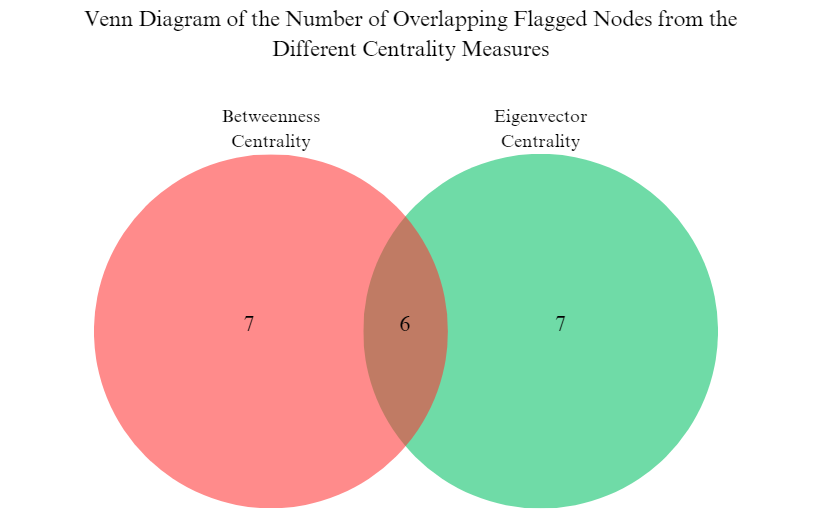
\includegraphics[scale=0.45]{venn}

\noindent{\small\textbf{Fig. 3.}  The red colored circle represents the number of Node IDs of the high betweenness centrality flagged nodes, and the green colored circle represents the number of Node IDs of the high eigenvector centrality flagged nodes.}

\bigskip
\noindent The nodes that were flagged as having high values for both centrality metrics are the nodes that need to be investigated further. 6 nodes were identified as having both high eigenvector and betweenness centralities out of the total 20 suspicious nodes that were flagged from the sample data. Therefore, the most influential nodes in the network according to both centrality metrics were the nodes with the following node IDs:

\begin{enumerate}
  \item node\_id = 367400
  \item node\_id = 378731
  \item node\_id = 160161
  \item node\_id = 652725
  \item node\_id = 26475
  \item node\_id = 76928
\end{enumerate}

\noindent Note: The results from this research question could be different if a new graph is created due to the sample of nodes being random

\subsection{Obtaining the Average Profile of a Fraudulent Account}

\normalfont
The average profile of a fraudulent account is as follows

\bigskip
\begin{tabular}{ | m{7cm} | m{3cm}|} 
  \hline
  \textbf{Attribute} & \textbf{Value} \\ 
  \hline
  payment\_type & 2 \\ 
  \hline
  keep\_alive\_session & 0 \\ 
  \hline
  foreign\_request & 0 \\
  \hline
  email\_is\_free & 1 \\
  \hline
  bank\_branch\_count\_8w & 210.1815 \\
  \hline
  zip\_count\_4w & 1648.506 \\
  \hline
  name\_email\_similarity & 0.3859064 \\
  \hline
  bank\_months\_count & 17.3637 \\
  \hline
  housing\_status & 1 \\
  \hline
  velocity\_6h & 5251.171 \\
  \hline
  phone\_home\_valid & 0 \\
  \hline
  current\_address\_months\_count & 30 \\
  \hline
\end{tabular}

\bigskip
\noindent{\small\textbf{Fig. 4.} Table representing the average profile of a fraudulent account based on the attributes of our dataset.}

\bigskip
\noindent Utilizing the average fraud node, we then set up thresholds for jaccard similarity and cosine similarity calculations. The thresholds for the similarity calculations were determined based on the characteristics of the dataset and the balance between meaningful detection and noise reduction. If the similarity score is above the threshold then an edge will be drawn between the typical fraud node and the actual node. A threshold of 0.5 was chosen for Jaccard similarity, meaning that at least 50\% of features, whether binary or numeric, needed to match; numeric features were considered to match if their difference was within a tolerance of 0.1. This ensures a focus on significant feature overlap. In the case of Cosine similarity, a stricter threshold of 0.7 was considered to capture strong alignment in feature vectors, considering both binary and numeric data. While Jaccard emphasizes exact matching at the feature level, Cosine captures more general structural alignment. Together, these thresholds were validated to effectively highlight fraudulent connections in the network without excessive noise.

\bigskip
\noindent
\begin{tabular}{ | m{5cm} | m{2.5cm}| m{3.2cm}|}
  \hline
  \textbf{Metric} & \textbf{Value} & \textbf{Percentage}\\ 
  \hline
  \textbf{Number of Jaccard Edges} & 0 & 0.00\%\\ 
  \hline
  \textbf{Number of Cosine Edges} & 148 & 2.15\%\\ 
  \hline
\end{tabular}

\noindent\textbf{Maximum possible edges: 6877}

\bigskip
\noindent{\small\textbf{Fig. 5.} The graph analysis indicates that the Jaccard similarity graph, with a maximum of 6877 possible edges, has 0 edges, which is 0.00\% of the total possible connections. On the other hand, the Cosine similarity graph contains 148 edges, accounting for only 2.15\% of the maximum possible edges.}

\subsection{Identifying Potential Fraudulent Groups}

After computing all edges and visualizing the graph to highlight the distribution of fraudulent and non-fraudulent nodes, we applied the Louvain method for community detection to group the nodes into clusters. The resulting graph is shown below.

\bigskip
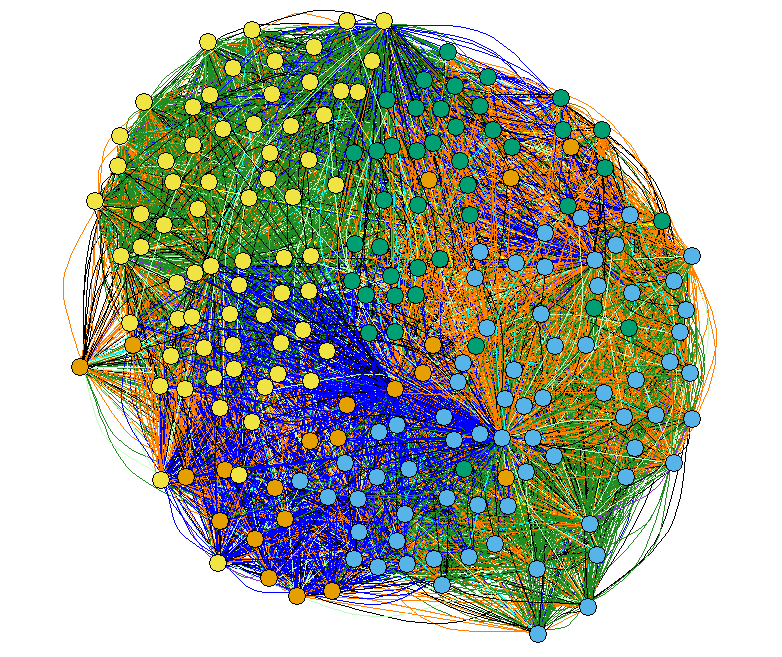
\includegraphics[scale=0.65]{q2comm}  

\bigskip
\noindent{\small\textbf{Fig. 6.} The above graph was created from a sample size of 200. The colors of the nodes represent the 4 communities identified during the community detection process. The edges represent the idea that 2 nodes are similar based on the various attributes of our dataset.}

\bigskip
\noindent The table below summarizes the average profiles and key statistics of the four communities, highlighting patterns and potential links to the characteristics of fraudulent nodes.

\bigskip
\noindent
\begin{tabular}{ | m{4.7cm} | m{1.8cm}| m{1.25cm}| m{1.25cm}| m{1.25cm}| m{1.25cm}|} 
  \hline
  \textbf{Attribute} & \textbf{Avg. Fraud} & \textbf{C1} & \textbf{C2} & \textbf{C3} & \textbf{C4}\\ 
  \hline
  payment\_type & 2 & 2 & 2 & 3 & 2 \\ 
  \hline
  keep\_alive\_session & 0 & 1 & 1 & 1 & 0 \\ 
  \hline
  foreign\_request & 0 & 0 & 0 & 0 & 0 \\
  \hline
  email\_is\_free & 1 & 1 & 1 & 1 & 1 \\
  \hline
  bank\_branch\_count\_8w & 210.18 & 234.92 & 234.92 & 100.17 & 183.48 \\
  \hline
  zip\_count\_4w & 1648.51 & 1614.70 & 1574.50 & 1500.80 & 1458.9 \\
  \hline
  name\_email\_similarity & 0.386 & 0.485 & 0.485 & 0.490 & 0.0215 \\
  \hline
  bank\_months\_count & 17.36 & 15.89 & 12.62 & 14.66 & 18.04 \\
  \hline
  housing\_status & 1 & 3 & 3 & 1 & 2 \\
  \hline
  velocity\_6h & 5251.171 & 5858.81 & 5165.11 & 5106.61 & 5235.64 \\
  \hline
  phone\_home\_valid & 0 & 0 & 0 & 0 & 0 \\
  \hline
  current\_address\_months\_count & 30 & 98 & 82 & 141 & 120 \\
  \hline
\end{tabular}

\bigskip
\noindent{\small\textbf{Fig. 7.} The table above shows the average profile of a fraudulent account, derived from the attributes in our dataset, alongside the average profiles of the four communities identified through the Louvain community analysis.}


\subsection{Finding Differences Between Fraudulent and Non-fraudulent Accounts}

\bigskip
\begin{tabular}{ | m{1.55cm} | m{1.65cm}| m{1.65cm}| m{1.65cm}| m{1.65cm}| m{1.65cm}| m{1.65cm}|}
  \hline
  \textbf{Metrics} & \textbf{Degree (Legit)} & \textbf{Degree (Fraud)} & \textbf{Eigen (L)} & \textbf{Eigen (F)} & \textbf{Jaccard (L)} & \textbf{Jaccard (F)}\\ 
  \hline
  \textbf{Mean} & 1380.840 & 1182.438 & 0.649 & 0.556 & 0.701 & 0.658\\ 
  \hline
\end{tabular}

\bigskip
\noindent{\small\textbf{Fig. 8.} Mean Degree Centrality, Eigenvector Centrality and Jaccard Similarity of fraud accounts (F) and legitimate accounts (L).}


\bigskip
\noindent
\begin{tabular}{ | m{1.55cm} | m{1.7cm}| m{1.7cm}| m{1.6cm}| m{1.6cm}| m{1.7cm}| m{1.7cm}|}
\hline
\textbf{Metrics} & \textbf{Closeness (Legit)} & \textbf{Closeness (Fraud)} & \textbf{Between (L)} & \textbf{Between (F)} & \textbf{Local Cluster (L)} & \textbf{Local Cluster (F)}\\ 
\hline
\textbf{Mean} & 1380.840 & 1182.438 & 0.649 & 0.556 & 0.701 & 0.658\\ 
\hline
\end{tabular}

\bigskip
\noindent{\small\textbf{Fig. 9.} Mean Closeness Centrality, Betweenness Centrality and Local Clustering Coefficient of fraud accounts (F) and legitimate accounts (L).}

\bigskip
\noindent Our results indicate that there are significant differences between fraudulent and legitimate nodes within the degree centrality, eigenvector centrality, betweenness centrality and Jaccard similarity. The closeness and local clustering metrics however have minute differences.
The most substantial discrepancy between means is within the Betweenness centrality, with a difference of 42.02\%, with legitimate nodes on average having much higher betweenness centrality. This is followed by the degree centrality means and eigenvector centrality means, which on average have differences of about 16.78\% and 16.72\%, respectively. Both the degree and eigenvector centralities are higher for Legitimate nodes. Legitimate nodes have a higher Jaccard centrality with a mean difference of 6.50\%. Closeness centrality and clustering centrality have the lowest mean difference with 2.94\% and 1.31\%, respectively; these differences are most likely too small to be considered substantial.


%Discussion start
\section{Discussion}

\subsection{Key Fraudulent Accounts}
The top 25 percentiles for each centrality measure was chosen as a threshold to focus investigations onto the nodes with abnormally high centrality values which flagged them as suspicious. These nodes that were flagged as suspicious may not themselves be fraudulent in reality but can be flagged as suspicious based on their connections to other nodes with high centrality scores within the network, and could possibly be collaborating with other nodes in the network to defraud the bank. The nodes that were flagged as having high eigenvector or betweenness centralities can be provided to domain experts as leads in a deep-dive investigation to see if any of the bank account applications held influence over the network by examining other attributes that were not a part of the dataset. The nodes that appeared as having high centralities for both metrics should be the first nodes to be examined to see if they were part of any fraud rings as a member or if they were leading fraud rings. The nodes with high betweenness centrality could be involved in fraud rings as middlemen and when a bank account request could be similar to many other account requests, and the node with the high betweenness centrality could provide the link between different account requests within a fraud ring, which could speed up fraud detection by providing more targeted node clusters that can be investigated. Using these centrality metrics should be done as one facet of the investigative process and should be used alongside the only method used to detect bank account fraud to prevent classifying nodes falsely as fraudulent. If data from transactions within these bank accounts that were being assessed for bank account fraud would have helped in zeroing in on more specific links to fraud rings, which is a limitation of this paper. Future research in a centrality metric-based approach to detecting bank account fraud can use neural networks to ingest the centrality metrics as new features as part of predicting bank account fraud. 

\subsection{Average Profile of a Fraudulent Account}
We can clearly see that, for both threshold values of 0.5 for Jaccard similarity and 0.7 for Cosine similarity, the typical fraud node does not provide a good indicator of the possible fraudulent applications. Most noticeably in the Jaccard similarity graph, the sparsity shows that these current thresholds are too conservative to reflect actual relationships between the typical fraud node and other nodes of the fraudulent class.That is to say, the normal fraud node will be unable to detect fraudulent behavior unless these thresholds are drastically lowered.The reason for this is that it cannot detect pattern/similarities based on the given threshold criteria. This suggests that we should either lower the threshold or come up with another method that better models the fraudulent activities within the network.

\subsection{Potential Fraudulent Groups}
In regard to the third research question, the analysis revealed four distinct communities within the network, with sizes ranging from 105 to 345 nodes. It should be noted however, that the modularity of the Louvain community structure was only 0.16, indicating that the clusters were likely just random groupings. The table comparing the average profile of a fraudulent account to the average profile of accounts in each community further confirms this. We can see that none of the four communities have a distinctly close relation to the average fraudulent account. It is important to note that the averages for all 4 of the communities are close to each other while the average fraudulent account is different from the rest. This is important because, considering the communities are mostly random, the distinctiveness of the average fraudulent profile highlights that it stands apart from these random groups. This demonstrates that the average fraudulent profile is notably different from a random grouping. Testing the entire dataset would require significantly more computing power or expensive software. However, doing so could provide a more definitive distinction and yield more concrete insights.

\subsection{Differences Between Fraudulent and Non-fraudulent Accounts}

Betweenness centrality, degree centrality, eigenvector centrality and the mean Jaccard similarity were determined to have the highest differences in means between fraudulent and legitimate nodes. Closeness centrality and clustering centrality had relatively insubstantial differences in means. 
The large discrepancy between mean betweenness suggests that the average legitimate node has 42.02\% more shortest paths going through it than the average fraudulent node. Although this result is the most substantial, betweenness centrality may not be the most appropriate metric to examine for this network compared to others. This is due to the fact that there is no flow of information or communication in an attribute-based network. Therefore, a node with high betweenness does not mean it controls the flow of information but that it is simply connected to more nodes based on shared attributes which results in more shortest paths passing through it. However, due to this substantial result it may still be worthwhile to investigate nodes with low betweenness centrality and compare their other metrics and attributes which have high capabilities for predicting fraudulent activity.
Mean degree centrality and eigenvector centrality are both on average approximately 17\% higher for legitimate nodes. This indicates that legitimate nodes had on average more connections and were connected to more nodes with high degree centrality; meaning that legitimate nodes share more similarities between attributes than fraudulent nodes. This implication is important, as it provides further evidence for the idea that there are indeed considerable differences between attributes of legitimate and fraudulent applications.
Legitimate nodes also had on average a higher Jaccard similarity coefficient than fraudulent applications. This means that legitimate nodes shared more common neighbours with other nodes, implying that they were better connected within the network. This result is consistent with the aforementioned metrics and implies that legitimate nodes share more common attributes.
Closeness centrality and the local clustering coefficient had little difference between legitimate and fraudulent nodes. A low discrepancy in closeness centrality most likely implies that although fraudulent nodes had less connections in terms of degree, they were still well connected in terms of reach to other nodes in the network. The local clustering coefficient had the lowest discrepancy of all the compared metrics. This means that there was very little difference in the likelihood of both legitimate and fraudulent nodes to form cliques with their neighbours. This is most likely due to the overall high connectivity of the network, if there is at least one edge between two neighbours of a node, a clique will be formed. This is likely to happen as both legitimate and fraudulent nodes have on average a higher degree than there are nodes present in the network.


%Conclusion start
\section{Conclusion}
To build a basis for fraud detection of bank applications using attribute-based networks we explored four relevant research topics. First, we examined the presence of key fraudulent players within the network by analyzing their eigenvector and betweenness centrality values in order to isolate influential nodes. We then determined the average profile of a fraudulent account and compared it against other nodes using the cosine and Jaccard similarity metrics to test the validity of using an average fraudulent profile as a means of fraud detection. Next, we applied the Louvain community detection algorithm to our network and compared the average profile of each community against the average profile of a fraudulent applicant to uncover potential fraudulent groups. Finally, we compared the means of six applicable network metrics for fraudulent and legitimate nodes to better understand their relationship and connectivity within the network.
Using eigenvector and betweenness centrality we were able to identify several influential nodes. Our results in identifying fraudulent activity using the typical fraud node were not conclusive, this was most likely due to the set threshold of the similarity metrics. We were also not able to identify fraudulent groups using the Louvain community detection algorithm, this is due to the detected groups being distinctly different from the typical fraudulent profile. We determined that 4 of the 6 compared metric means were substantially different between legitimate and fraudulent nodes.
These results indicate that conventional network analysis metrics and algorithms may prove useful in identifying fraudulent activity. However, further research and resources are needed to provide conclusive results. One of the main limitations of this analysis was inadequate computational power. We believe that a more exhaustive dataset combined with greater computational capabilities can provide conclusive results for the methods explored in this analysis. These methods may also prove useful in real-world applications, especially when combined with existing fraud detection techniques.

\newpage
%
% ---- Bibliography ----
%
\begin{thebibliography}{6}
%

\bibitem {smit:wat}
Dataset citation
@article{jesusTurningTablesBiased2022,
  title={Turning the {{Tables}}: {{Biased}}, {{Imbalanced}}, {{Dynamic Tabular Datasets}} for {{ML Evaluation}}},
  author={Jesus, S{\'e}rgio and Pombal, Jos{\'e} and Alves, Duarte and Cruz, Andr{\'e} and Saleiro, Pedro and Ribeiro, Rita P. and Gama, Jo{\~a}o and Bizarro, Pedro},
  journal={Advances in Neural Information Processing Systems},
  year={2022}
}

\bibitem {gran:nob:lam}
F. Grando, D. Noble and L. C. Lamb, "An Analysis of Centrality Measures for Complex and Social Networks," 2016 IEEE Global Communications Conference (GLOBECOM), Washington, DC, USA, 2016, pp. 1-6, doi: 10.1109/GLOCOM.2016.7841580. keywords: {Measurement;Complex networks;Correlation;Social network services;Informatics;Correlation coefficient;Analytical models},

\bibitem {czaj:fitz}
Motie, Soroor, and Bijan Raahemi. "Financial fraud detection using graph neural networks: A systematic review." Expert Systems with Applications 240 (2024): 122156.

\bibitem {gir:bho}
Girish, K.K., Bhowmik, B. (2024). Historical Analysis of Financial Fraud and Its Future. In: Thampi, S.M., Hu, J., Das, A.K., Mathew, J., Tripathi, S. (eds) Applied Soft Computing and Communication Networks. ACN 2023. Lecture Notes in Networks and Systems, vol 966. Springer, Singapore. \url{https://doi.org/10.1007/978-981-97-2004-0_4}

\bibitem {fo:kes:nic:tue}
Deprez, Bruno, et al. "Network analytics for insurance fraud detection: a critical case study." European Actuarial Journal (2024): 1-26.

\bibitem {nor:ism:zur:hen}
Normah Omar , Ismail bin Mohamed , Zuraidah Mohd Sanusi and Hendi Yogi Prabowo (2014). Understanding Social Network Analysis (SNA) In Fraud Detection. Recent Trends in Social and Behaviour Sciences \url{https://www.researchgate.net/profile/Normah-Omar/publication/300376345_Understanding_Social_Network_Analysis_SNA_in_fraud_detection/links/5874560508ae8fce4924ff57/Understanding-Social-Network-Analysis-SNA-in-fraud-detection.pdf}


\end{thebibliography}
\end{document}
